\begin{exercicebox}[   \it{(QCM)} \hspace*{\fill}\bb{4pts}]
    \bb{Entourer la bonne réponse}\\
    \bb{1)} On a demandé à un groupe de personne leur couleur préférée. Voici leurs
    réponses : 

    \begin{minipage}{0.65\textwidth}
    \begin{center}
    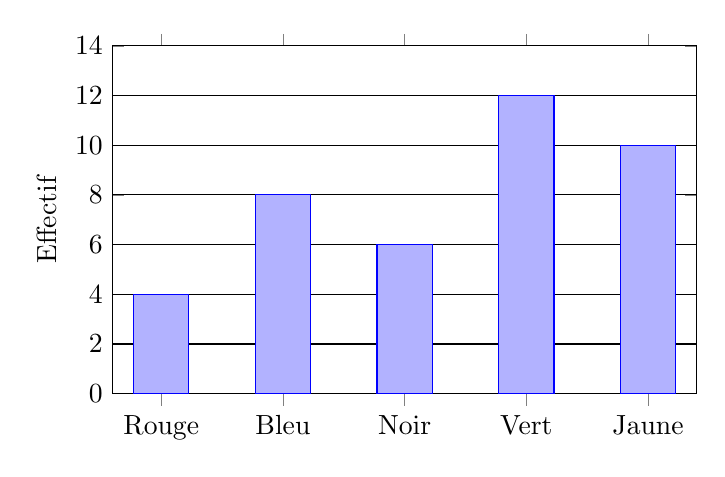
\begin{tikzpicture}
    \begin{axis}[
        ybar,
        ylabel={Effectif},
        ytick distance=2,
        ymin=0,
        ymax=14,
        xtick={1,2,3,4, 5},
        xticklabels={Rouge,Bleu,Noir,Vert, Jaune},
        bar width=20pt,
        width=9cm,
        height=6cm,
    ]
    \draw[step=2.0, black] (0,0) grid (14,14);
    \addplot coordinates {
        (1,4)
        (2,8)
        (3,6)
        (4,12)
        (5,10)
    };
    \end{axis}
    \end{tikzpicture}
    \end{center}
    \end{minipage}
    \begin{minipage}{0.3\textwidth}
        L'effectif total est:
        \begin{center}
        a) 40 \hspace{1cm} b) 56\hspace{1cm} c) 5
        \end{center}
    \end{minipage}

    \vspace{12pt}
    \bb{2)} Le professeur d'EPS a relevé les distance atteintes par ses 23 élèves au
    saut en longueur
    \begin{center}
    \begin{tabular}{|c|c|c|c|c|}
        \hline
        \bb{Longueur (m)}  & 3 & 3.5 & 4 & 4.5  \\ \hline
        \bb{Effectif} & 8 & 7 &  & 3  \\ 
        \hline
    \end{tabular}
    \end{center}

    \begin{minipage}{0.49\textwidth}
        a) L'effectif des élèves qui ont atteint 4m est: 
        \begin{center}
            2 \hspace{1cm} 5 \hspace{1cm} On ne peut pas savoir\\
        \end{center}
    \end{minipage}
    \vline
    \hfill
    \begin{minipage}{0.49\textwidth}
    b) La fréquence de ceux qui ont atteint 3m est:
        \begin{center}
             $\dfrac{3}{8}$\hspace{1cm} $25\%$\hspace{1cm} $\dfrac{8}{23}$
        \end{center}
    \end{minipage}
    
    \vspace{20pt}
    \begin{minipage}{0.49\textwidth}
    \bb{3)} Voici les notes de Romain en anglais ce trimestre : \bb{8; 14; 15; 7}. Sa moyenne trimestrielle en anglais est: 
        \begin{center}
        \hspace{1cm}a) 10 \hspace{1cm}a) 11\hspace{1cm}c) 12 
        \end{center}

    \bb{4)} Sur le diagramme circulaire, le secteur marqué d'un point d'interrogation
    représente un pourcentage de :  
        \begin{center}
            a) 20\% \hspace{1cm}b) 45\%\hspace{1cm}c) 55\%
        \end{center}
    \hfill
    \end{minipage}
    \begin{minipage}{0.49\textwidth}
        \begin{center}
        \includegraphics[scale=0.4]{ASSETS/circulaire}
        \end{center}
    \end{minipage}


 

\end{exercicebox}

